\documentclass[conference]{IEEEtran}

%\IEEEoverridecommandlockouts
% The preceding line is only needed to identify funding in the first footnote. If that is unneeded, please comment it out.

\usepackage{cite}
\usepackage{amsmath,amssymb,amsfonts}
\usepackage{algorithmic}
\usepackage{graphicx}
\usepackage{textcomp}
\usepackage{xcolor}
\usepackage[]{hyperref}
\usepackage{subfigure}
\usepackage{booktabs}

\graphicspath{{./figures/}}

%\def\BibTeX{{\rm B\kern-.05em{\sc i\kern-.025em b}\kern-.08em
%    T\kern-.1667em\lower.7ex\hbox{E}\kern-.125emX}}
\newcommand{\cheng}[1]{{\textcolor{red}{ #1}}}
% correct bad hyphenation here
\hyphenation{}



\begin{document}

% paper title
% Titles are generally capitalized except for words such as a, an, and, as,
% at, but, by, for, in, nor, of, on, or, the, to and up, which are usually
% not capitalized unless they are the first or last word of the title.
% Linebreaks \\ can be used within to get better formatting as desired.
% Do not put math or special symbols in the title.
\title{Persistent Fault Analysis of Convolutional Neural Networks on FPGA-based Acceleration System}

% author info
%\author{\IEEEauthorblockN{1\textsuperscript{st} Given Name Surname}
%\IEEEauthorblockA{\textit{dept. name of organization (of Aff.)} \\
%\textit{name of organization (of Aff.)}\\
%City, Country \\
%email address}
%\and
%\IEEEauthorblockN{2\textsuperscript{nd} Given Name Surname}
%\IEEEauthorblockA{\textit{dept. name of organization (of Aff.)} \\
%\textit{name of organization (of Aff.)}\\
%City, Country \\
%email address}
%\and
%\IEEEauthorblockN{3\textsuperscript{rd} Given Name Surname}
%\IEEEauthorblockA{\textit{dept. name of organization (of Aff.)} \\
%\textit{name of organization (of Aff.)}\\
%City, Country \\
%email address}
%\and
%\IEEEauthorblockN{4\textsuperscript{th} Given Name Surname}
%\IEEEauthorblockA{\textit{dept. name of organization (of Aff.)} \\
%\textit{name of organization (of Aff.)}\\
%City, Country \\
%email address}
%\and
%\IEEEauthorblockN{5\textsuperscript{th} Given Name Surname}
%\IEEEauthorblockA{\textit{dept. name of organization (of Aff.)} \\
%\textit{name of organization (of Aff.)}\\
%City, Country \\
%email address}
%\and
%\IEEEauthorblockN{6\textsuperscript{th} Given Name Surname}
%\IEEEauthorblockA{\textit{dept. name of organization (of Aff.)} \\
%\textit{name of organization (of Aff.)}\\
%City, Country \\
%email address}
%}

% make the title area
\maketitle


% As a general rule, do not put math, special symbols or citations
% in the abstract
\begin{abstract}
    Deep neural network (DNN) is making continuous breakthroughs 
    in massive domains of applications and is increasingly 
    deployed on customized DNN accelerators for both the 
    higher performance and energy efficiency. While the 
    increasing hardware failures caused by the shrinking semiconductor 
    technology may have substantial influence on the accelerators and 
    improving the resilience of the neural network execution becomes a great 
    challenge especially to mission-critical applications such as self-driving 
    and medical diagnose. The reliability analysis of the neural 
    network execution is a key step to understand and alleviate the influence 
    of the hardware failures, and thus is highly demanded. 
    
    Prior works typically focus on the computing errors of neural networks caused by 
    hardware faults with simulation, but there is still a lack of fault 
    analysis from a system point of view. For instance, the consequences of 
    the system such as system stall are also critical to resilient 
    neural network execution. In this work, we implemented a 
    representative neural network accelerator as well as fault injection modules 
    on a Xilinx ARM-FPGA platform (ZC706). Then we conducted comprehensive fault 
    analysis of the system using four typical neural network models
    from different system angles including system functionality, 
    fault coverage, and input variation as well as prediction 
    accuracy loss. Based on the analysis, we find that system stall 
    caused by hardware faults is non-trivial to the system reliability 
    and further propose an efficient approach to alleviate it with negligible 
    hardware overhead. 
    
\end{abstract}


%\begin{IEEEkeywords}
    % keyword1, keyword2, keyword3, keyword4, keyword5
%\end{IEEEkeywords}


% For peer review papers, you can put extra information on the cover
% page as needed:
% \ifCLASSOPTIONpeerreview
% \begin{center} \bfseries EDICS Category: 3-BBND \end{center}
% \fi
%
% For peerreview papers, this IEEEtran command inserts a page break and
% creates the second title. It will be ignored for other modes.
\IEEEpeerreviewmaketitle

\section{Introduction}
Offloading compute intensive nested loops to FPGA accelerators has 
been demonstrated as an effective way of performance 
acceleration across various application domains\cite{Chung2010}. 
However, the design productivity of developing such accelerators 
remains relatively low and it has become a major obstacle that 
hinders the wide adoption of FPGAs as compute engines. Although the use of 
high level synthesis (HLS) tools which allow the application designers to 
focus on high level functionality instead of low-level implementation details alleviates 
this shortcoming \cite{cong2011high}, the lengthy low-level FPGA implementation process 
greatly limits the number of compile-debug-edit cycles per day and dramatically 
affects the overall design productivity. 

To approach the above design productivity problem, 
researchers have recently turned to the use of virtual FPGA overlay 
architectures \cite{Grant2011Malibu,ZUMA2012,mesh-FUs,
ferreira2011fpga, kissler2006dynamically,scgra}. When combined properly to 
high level compilation tools, the overlay architecture based design methods 
are able to produce high-performance accelerators at near software 
compilation speed, but at the cost of hardware overhead, power and even performance.
By customizing the architectures of these \emph{virtual} 
overlays for a target user design, in theory, it is 
possible to significantly improve the performance-energy of the 
resulting accelerator. In practice, however, navigating through a 
labyrinth of architectural and compilation parameters to fine-tune 
an accelerator's performance-energy is a slow and non-trivial process. 
To require a user to manually explore such vast design space is going 
to counteract the productivity benefit of the utilizing overlay 
in the first place.

To obtain both high design productivity and advantages of 
application-specific customization, we have developed a 
soft CGRA (SCGRA) overlay based nested loop acceleration design 
framework. This framework targets a hybrid CPU-FPGA computing system where 
nested loop compute kernels expressed in high-level languages are compiled and 
executed on the SCGRA overlay built on top of FPGAs while the rest of the 
user application remains running on the host CPU. Given high-level design 
goals and design constraints, the framework automatically explores the 
design space and customizes architectural parameters specifically to the 
user application. In addition, the framework also exploits loop unrolling 
and hardware-software communication strategies in combination 
with buffer sizing and partition as performance enhancing techniques.
Once the design goals and constraints are fulfilled, the 
corresponding hardware accelerator and communication interface 
are generated and both the hardware accelerator and software 
are compiled to the hybrid CPU-FPGA system.  

As demonstrated in previous work, both the compilation from nested 
loops to the SCGRA overlay \cite{scgra} and the SCGRA overlay 
implementation \cite{ROB2014} are fast. Meanwhile, the SCGRA 
overlay is highly pipelined and has quite regular tiling structure, 
which makes the hardware overhead, power consumption and even implementation frequency 
highly predictable. Therefore, a multitude of design metrics such as performance 
and energy consumption can be accurately estimated using analytical models when the 
overlay scheduling result is available. And the nested loop specific acceleration problem can be 
reduced to a sub design space exploration centering an NP-complete SCGRA scheduling and 
a following customization with all the potential configurations well estimated. 
While the overlay scheduling depends on much less design parameters, the overall 
customization can be dramatically simplified. Accordingly, the overall design 
framework achieves both rapid compilation and fast application specific 
customization and ensures high design productivity and high performance of the resulting
accelerators at the same time.  

We performed a series of experiments to evaluate the efficiency 
and quality of the proposed design framework using a real-world 
benchmark. Compared to an exhaustive search, the proposed 
customization achieves similar results while reducing its 
runtime by 2 orders of magnitude on average. When compared to 
HLS implementations with moderate manual optimizations that can 
reasonably be expected from a novice user,  
the customized accelerators produced using the proposed framework 
has demonstrated competitive performance as well. 

With that, we consider the main contribution of this work is in the following areas:
\begin{itemize}[nosep]
\item We have developed a rapid customization framework that 
    performs automatic design parameter tuning for SCGRA overlay based 
    nested loop acceleration on a hybrid CPU-FPGA computing system. 
    The result is comparable to an exhaustive design space search while 
    it runs at a fraction of time.
\item We have developed a parametric regular SCGRA overlay template. It can be used 
    to generate FPGA accelerators with predictable implementation 
    frequency, hardware overhead and power consumption, which is essential to 
    both the rapid compilation and customization.
\item We have developed a hierarchy on-chip buffer. It allows flexible 
    buffer partition and makes good use of the efficient lock-step computation 
    of the SCGRA overlay.
\end{itemize}

In \secref{sec:relatedwork}, related work is briefly introduced. 
The overall automatic nested loop acceleration framework is illustrated 
in \secref{sec:acc-framework}. Then SCGRA overlay based FPGA accelerator 
is illustrated in \secref{sec:scgra} and the application-specific customization 
method is further detailed in \secref{sec:customization-method}. 
Experimental results are presented in \secref{sec:result} and limitations are 
discussed in \secref{sec:limitations}. Finally, the paper is 
concluded in \secref{sec:conclusion}.



\section{Background}\label{sec:background}
Hardware faults in the DNN accelerators are the major sources of 
the unreliability. The influence of faults is closely related with 
the micro architecture of the DNN accelerators. To help understand and 
investigate the fault tolerance of the accelerators, we take a typical 
DNN accelerator with a regular 2D processing element (PE) array as an example 
and elaborate its architecture in this section.

The representative DNN accelerator is illustrated in 
Figure ~\ref{fig:npu-arch}. It adopts output stationary data flow 
to map computing such as convolution to the 2D computing array. 
Each PE in the array performs all the operations 
required to yield an output activation. While each PE has only a 
single multiplier and accumulator, it accumulates all the input 
activations in a filter window sequentially. To that end, weights 
are fed to the first column of the PE array in parallel and flow 
through PEs from left to right to ensure that all PEs operate in full 
scale. While input activations are organized in a batch and sent 
to one column of PE every cycle, each PE in the column shares the 
same input data through broadcasting and it takes 
each PE multiple cycles to complete the accumulation. 
During this period, more batched input activations 
can be read and sent to the next column of PEs along with 
the movement of the weights. Output activations flow 
from right to left in column-wise. Eventually, each row of the PEs
array produces a set of sequential output activations in 
the same row of one output feature map on y-axis. 
Each column of the PEs produces the output activations 
belonging to different output feature maps but the 
same position in z-axis. The architecture along with the 
compact data flow achieves high data reuse under limited 
on-chip buffer bandwidth provision. 

\begin{figure}
    \center{\includegraphics[width=0.8\linewidth]{npu-arch}}
    \caption{Typical DNN accelerator architecture}
\vspace{-0.5em}
\label{fig:npu-arch}
\end{figure}

Both convolution layer and full connection layer can be mapped to the 
array efficiently. While pooling and other non-linear activation functions 
such as sigmoid will be performed right after the computing-intensive 
layers like convolution layer in a module named XPE such that 
the data movement between the two layers can be reduced. 
All the neural network operations can be mapped to the 
accelerator. To map diverse neural 
network models with different combination of layers and parameters such as 
stride size, kernel size, and input/output feature map size, we define 
a set of instructions to generate appropriate control signals 
for different neural network operations. Each neural network 
will be compiled to a series of instructions and executed sequentially. 
In addition, neural network input features and weights 
are usually larger than the on-chip buffers and PE array size, 
so they must be tiled and the tiles need to be scheduled to 
obtain efficient execution on the accelerator. To enable fine-grained 
optimizations, each instruction only handles operations of 
a single tile. Thus, tiling is performed during model
compilation and it is transparent to the instructions.

Table ~\ref{tab:instrction-set} shows the instruction set of the neural 
network accelerator. It adopts 64-bit fixed length encoding 
and consists of four types of instructions including parameter 
setup, calculation, data movement and control. The parameter setup 
category defines the input/output feature size, kernel size, 
Q-code, and DMA parameter. Calculation 
category includes different operations in neural networks such as 
convolution, full connection, pooling, addition, softmax, 
dot-accumulation and activation function etc. Data movement category
includes three instructions which move a block of data 
from DRAM to buffer, buffer to DRAM and buffer to buffer 
respectively. Finally, control category includes three instructions which are 
Jump, Stop and Nop. Jump instruction is mainly used for repeated 
execution. Stop is used to terminate the execution of the accelerator.
Nop is used to resolve the data dependency between sequential 
instructions.

\begin{table}
    \centering
    \caption{Instruction Set of the DNN Accelerator}
    \label{tab:instrction-set}
    \begin{tabular}{cp{0.6\columnwidth}}
        \toprule
        Instruction Type & Description \\
        \midrule
        Parameter setup & Setup parameters for the computing operations such as the input/output feature size, kernel size, Q-code, and DMA options\\
        \midrule
        Calculation & Performs various neural network operations such as convolution, full connection, pooling, addition, softmax, dot-accumulation and activation function \\
        \midrule
        Data movement & Move a block of data from buffer to buffer, buffer to DRAM and DRAM to buffer.\\
        \midrule
        Control & Control the execution of the accelerator such as Jump, Nop and Stop\\
    \bottomrule
    \end{tabular}
    \vspace{-1em}
\end{table}

The neural network accelerator architecture is general enough to support 
various neural network models. In addition, it typically works along 
with a general purposed processor and has an AXI slave port that allows 
configuration and controlling from the attached processor. It assumes 
the input data, weight and output data are stored in DRAM that can be 
accessed directly.
\section{Faulty DNN Accelerator Analysis Platform and System Problems}
\label{sec:fault-analysis}
\subsection{Fault Analysis Platform}
To conduct system fault analysis on a realistic system, we build a fault 
analysis platform on Xilinx Zynq (ARM-FPGA) as shown in 
Figure \ref{fig:fault-analysis-overview}. It includes a full FPGA-based 
neural network acceleration system that has both a general purposed 
processor (ARM) and a DNN accelerator implemented on the FPGA. 
Typically, the processor sets up the neural network parameters through 
an AXI configuration port and allocates specific memory 
space for instruction/input/output/weight data. Then it can 
start the DNN accelerator. When the computing is done, DNN accelerator 
will notify the processor with interruption to collect the result from the 
shared DRAM. 

\begin{figure}
    \center{\includegraphics[width=0.99\linewidth]{system-overview}}
    \caption{Overview of the fault analysis system}
\vspace{-0.5em}
\label{fig:fault-analysis-overview}
\end{figure}

On top of the baseline FPGA-based neural network acceleration, 
we develop a configurable fault injection scheme. The injection data path 
is marked with the orange arrows and located on both the ARM processor and 
FPGA. On the arm processor part, we implement the fault models such as bit-flip, 
stuck-at-0, stuck-at-1, multiple-bit upset etc. and generate a set of bit errors 
based on a random fault distribution model. Then the errors are sent to 
the FPGA-based DNN accelerator from an AXI port. The errors are distributed to 
both FPGA configuration memory and the block RAM evenly based on the memory size.
Nevertheless, the error injection data paths to FPGA configuration memory 
and on-chip block RAM are quite different.

For FPGA configuration memory, we take advantage of Xilinx ICAP 
port \cite{UG953}, which allows user logic to access configuration 
memory, to inject errors. While Xilinx FPGA bitstream is organized 
as frames and each frame includes configuration bits of a block of 
FPGA, we randomly choose the frame and the number of bits for each 
bit error injection. The error can be located at any place of the 
FPGA configuration memory including the regions that are not utilized.
When the position of an error is determined, we read the whole frame 
out of the configuration memory via AXI port of AXI-HWICAP \cite{PG134}, 
change the victim bit in the frame, and write it back to the configuration 
memory \cite{UG470}. This can be done on the ARM processor either before the fault 
analysis or during the fault analysis. Thereby, the fault injection 
to FPGA configuration memory can either be performed with online 
manner or offline manner.

For the block RAM, we develop an error mask (Err. Mask) which can be 
added to a block RAM. The mask will not change the interface nor the 
pipelining of the original block RAM, but it has an AXI slace port
allowing ARM processor to flip a bit of any data in the block RAM 
during reading. Figure \ref{fig:error-mask} shows the design of the error mask.
Basically, it has a set of address and mask registers that can be configured 
using the attached AXI slave port. The addresses in the registers represent 
the position of errors to be injected while the corresponding masks 
keep the exact error bits. When there is a read request coming 
to the block RAM, the read address will be compared with all 
the addresses in the registers. when there is an address match, 
the data read from the block RAM will be XORed with the mask.
Then the result will be used as the output of the block RAM 
affected with injected errors. Since the registers in the error mask 
can either be configured runtime, the error injection to 
the block RAM can also be done in both an offline manner 
and an online manner.

\begin{figure}
    \center{\includegraphics[width=0.8\linewidth]{error-mask}}
    \caption{Error mask for fault injection to buffers}
\vspace{-0.5em}
\label{fig:error-mask}
\end{figure}

Another important part of the fault analysis platform is the result 
collection and comparison. While the results of the neural networks 
running on the DNN accelerator are stored in the DRAM, it is 
Finally, we want to emphasize that the fault injection hardware is 
attached to the ARM processor with AXI slave port. With a 
driver, the AXI fault injection can be triggered in software running 
on the ARM processor.

\subsection{Consequences of faults in DNN accelerators}
\subsection{Fault model}
In our error injection design, the error injection to the 
configuration memory is global, regardless of whether the 
configuration block corresponding to the configuration bit 
is used. The injection of BRAM is designed to only inject 
errors into the BRAM used by user logic. In order to make 
the error injection as consistent as possible with the 
error generation under the radiation condition, we 
calculate the proportional relationship between the 
configuration memory and the block memory used.

Refer to Xilinx official documentations, the configuration 
Bitstream length of the XC7Z045 SoC used by the Zynq-7000 
SoC ZC706 Evaluation Board is 106,571,232 bits \cite{UG585}, which can 
be approximately regarded as the number of configured 
memory bits, and the available block memory is 20,090,880 
bits \cite{DS190}. After conversion, the accessible configuration memory 
accounted for about 84.14\%, while the block memory 
accounted for 15.86\%. In the NPU under test, the actual 
use of BRAM accounts for 30.43\% of the total bits, that is, 
4.83\% of the total bits of SRAM.

Based on the above calculations, we determined that the 
location where a single random error occurred would have an 
84.14\% chance of appearing in configuration memory and a 
4.83\% chance of appearing in actual used BRAM. When errors 
occur in these two areas, they can have an impact on the 
behavior and results of the system. In addition, the error 
will have an 11.03\% chance of appearing in unused BRAM, 
which will not have any impact on the system.

Before each Neural Network prediction, we randomly inject 
certain number of fixed upset errors into the system, which 
will persist in the process of Neural Network prediction 
until the end of prediction or timeout failure. After one 
prediction is performed, the errors in the system are 
recovered and the next random error injection and 
prediction is performed.


\subsection{Error Assessment}
We chose Neural Networks in four different application 
scenarios and try to analyze the differences of error 
tolerance in different application scenarios and networks. 
The four network applications include ResNet network for 
image classification, YOLO system for target detection, 
LSTM network for voice classification, and DCGAN network 
for image generation. We will evaluate their fault 
tolerance from accuracy and output consistency.

Neural Network accelerators injected with hardware errors 
may produce unexpected conditions. We define the system 
halt situation, which refers to a serious error in the 
system, or working improperly. such as unable to read and 
write registers, timeout, abnormal short runtime, etc. When 
the system halts, we need to reset the FPGA and restart the 
system. System halt situations are considered the result of 
errors in the evaluation of network accuracy and are listed 
separately in the output consistency.

Network accuracy refers to the overall accuracy of the 
network when performing corresponding tasks, such as the 
accuracy of 20,000 image recognition. When there are errors 
in the operation, the accuracy of the network will show a 
downward trend. For classification networks including 
ResNet and LSTM, top-5 accuracy is used to evaluate their 
accuracy, and for the YOLO system, mAP is adopted.

Output consistency is the difference between the result of 
running with errors injected and the result of normal 
running. We ran the corresponding data set when no errors 
are injected into each network at first, and defined the 
results as standard output. The results of Neural Networks 
prediction injected with errors are divided into two 
categories: result with deviation and result match. Result 
with deviation refers to system works properly with output 
differently from standard output. Result match means that 
the system works properly and the outputs are still 
standard output.

For the result with deviation case, we define its deviation 
quantitatively and further subdivide the result. Due to the 
different application functions of each network, the 
evaluation criteria of deviation are also different. For 
YOLO system, the result is the target detection bounding 
box, and when the detection result does not match the 
standard output in object type, it is defined as detection 
result error. When the result target type is consistent, 
the error is defined as the intersection area of the error 
output and the standard output divided by the area of the 
union. Target types not match for one single level, the two 
do not overlap with each other for one level, and then each 
20\% is divided into one level. For ResNet and LSTM, the 
outputs are top-5 labels. When the error output is not 
completely consistent with the standard output, the number 
of elements in the intersection of the two is taken, and 
divide the levels refer to the number. For DCGAN, we used 
the universal SSIM standard, and divided it into six levels 
according to the actual visual effects: 0~10\%, almost 
impossible to recognize; 10~20\%, barely visible; 20~50\%, 
with large deformation or distortion; 50~80\% with partial 
deformation or distortion; 80~90\%, small deformation or 
distortion can be seen; 90~100\%, almost no deformation or 
distortion is visible.

\section{Experiment} \label{sec:experiment}
We seek to understand the influence of persistent errors on 
FPGA-based neural network acceleration system. Particularly, 
we try to analyze the influence from a system point of view
and figure out the underlying reasons for severe system problems 
such as system stall and dramatic prediction accuracy loss. 

\subsection{Device and Environment}
Xilinx Zynq-7000 SoC ZC706 Evaluation Board will be used in 
the experiments’ hardware implementation. It has 
appropriate hardware resources and is easy to develop and 
use. The hardware design and Bitstream file compilation 
were completed using the upper computer with Intel Core 
i7-6700 processor and 2x8GB DDR4 2400MHz memory. The system 
environment used was Ubuntu 16.04 LTS version, and Xilinx 
Vivado Design Suite and Xilinx Software Development Kits 
version 2017.4.

The hardware resource utilization of the error analysis 
platform implementation on ZC706 is shown in Table \ref{tab:utilization report}.

The four models cover a broad range of applications.
Yolo represent a typical neural network model for object detection \cite{redmon2016yolo9000}, 
Resent is a widely adopted neural network model for classification \cite{He_2016_CVPR}, 
LSTM is the mostly used neural network model for audio classification 
tasks \cite{sak2014long}, and DCGAN stands for a typical neural network model for 
generative tasks \cite{radford2015unsupervised}. 

Despite the widespread adoption of deep learning 
neural network on various applications, it is particularly 
successful in four categories of tasks including object detection, 
object classification, voice recognition and style transfer.
Among a great number of neural network models,
Yolo, Resnet, LSTM and DCGAN are four typical neural networks 
that are comprehensively explored to handle the four computing 
tasks respectively. 

\begin{table}
    \centering
    \caption{Utilization Report of Fault Analysis Platform}
    \label{tab:utilization report}
    \begin{tabular}{cccc}
        \toprule
        Resource & Utilization & Available & Utilization Percentage \\
        \midrule
            LUT & 122618 & 218600 & 56.09\% \\
            LUTRAM & 185 & 70400 & 0.26\% \\
            FF & 84641 & 437200 & 19.36\% \\
            BRAM & 203 & 545 & 37.25\% \\
            DSP & 297 & 900 & 33\% \\
            MMCM & 1 & 8 & 12.5\% \\
        \bottomrule
    \end{tabular}
\vspace{-1em}
\end{table}

\subsection{Overview}
We hope to explore the possible consequences of errors, the 
fault-tolerant ability of different applications and the 
influence of different error locations of accelerators, 
which can provide meaningful references for the subsequent 
network optimization and the fault-tolerant design of 
accelerators.

We conducted five sets of experiments, which explained the 
influence of single error on different networks, the 
difference of fault tolerance ability of different 
applications, the error classification of different 
applications, the influence of different accelerator units 
and whether the input data affected the error representation.


\subsection{Error Consequences and Coverage}
First, we conducted single-bit random error injection 
experiments for different applications, and conducted 
20,000 runs for each application, to analyze the proportion 
of single-bit random error shielded in the system and the 
possible influence of single-bit random error on the 
accelerator system. Figure \ref{fig:lab1-error-rate} shows the 
percentage of application errors caused by a single-bit 
random hardware error. In the experiment, we found that 
more than 90\% of the errors were masked by software or 
hardware. However, while most errors are masked without 
impact to the operation, a single-bit error can lead to 
serious exceptions, including system halt, serious 
deviation in results, and so on. In addition, LSTM network 
has a better fault tolerance performance than other three 
networks, and the proportion of the influence caused by 
single error of the other three networks is about 5~7 times 
that of LSTM. According to our analysis, this is because 
LSTM network is smaller than other networks and uses less 
storage and computing resources.

\begin{figure}
	\center{\includegraphics[width=0.9\linewidth]{lab1-error-rate}}
    \caption{Application error rate caused by single-bit random hardware error}
\label{fig:lab1-error-rate}
\vspace{-0.5em}
\end{figure}


\subsection{Effect of Error Number}
We completed a single run with errors injected number of 
powers of 2, with 20,000 runs for each network. In general, 
the proportion of system halt and result with deviation 
increases with the number of errors, and the accuracy of 
application decreases. Figure \ref{fig:lab2_2} show the proportion of 
system halt and result deviation, and Figure \ref{fig:lab2-network-accuracy} shows the 
accuracy of each network. We found that the influence of 
multiple errors on the accelerator was obvious and far 
beyond our expectation. The Neural Network accelerator is 
still vulnerable to errors. By the time we injected 16 
errors in a single run, the system halt rate was more than 
1\%, means it took more time to restore the system than to 
run it. From the perspective of network accuracy, take YOLO 
system as an example, its mAP decreases by 8.95\% when it 
runs with 16 errors, means the application function of the 
system is also seriously affected.

The result with deviation proportion of different networks 
appears differently with the increase of error number. When 
16 errors are injected, LSTM network still has a small 
result deviation proportion due to its small network 
structure. The proportion of YOLO system is very high, with 
about 70\% of the results showing errors. ResNet is 
relatively low, with only about 35\% result deviation. 
DCGAN network is in between, and about 50\% of the results 
have numerical errors. We believe that the result deviation 
may be related to the structure of the output. The output 
of YOLO system contains more information such as object 
type, location and size of bounding box, etc., and the 
output of ResNet is simple sorting, while the simple output 
is obviously less susceptible to errors.

\begin{figure}
	\center{\includegraphics[width=0.85\linewidth]{lab2-network-accuracy}}
    \caption{Network accuracy versus error number}
\label{fig:lab2-network-accuracy}
\vspace{-0.5em}
\end{figure}

\begin{figure}
    \centering
    \subfigure[System halt]{\includegraphics[width=0.45\linewidth]{lab2-system-halt}}
    \subfigure[Result with deviation]{\includegraphics[width=0.45\linewidth]{lab2-result-with-deviation}}
    \caption{Abnormal situation proportion versus error number}
\label{fig:lab2_2}
\vspace{-0.5em}
\end{figure}


\subsection{Details of Result with Deviation}

\begin{figure*}
    \centering
    \subfigure[YOLO]{\includegraphics[height=0.12\textheight]{lab3-yolo}}
    \subfigure[ResNet]{\includegraphics[height=0.12\textheight]{lab3-resnet}}
    \subfigure[LSTM]{\includegraphics[height=0.12\textheight]{lab3-lstm}}
    \subfigure[DCGAN]{\includegraphics[height=0.12\textheight]{lab3-dcgan}}
\caption{Distribution of result with deviation situations}
\label{fig:lab3}
\vspace{-0.5em}
\end{figure*}

\begin{figure*}
    \centering
    \subfigure[YOLO]{\includegraphics[height=0.10\textheight]{lab4-yolo}}
    \subfigure[ResNet]{\includegraphics[height=0.10\textheight]{lab4-resnet}}
    \subfigure[LSTM]{\includegraphics[height=0.10\textheight]{lab4-lstm}}
    \subfigure[DCGAN]{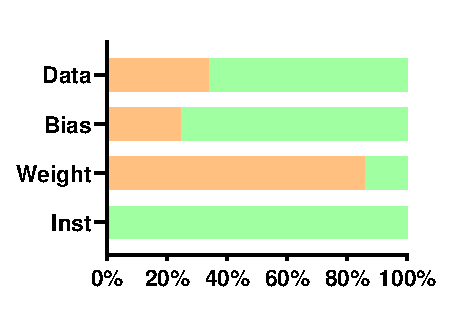
\includegraphics[height=0.10\textheight]{lab4-dcgan}}
    \includegraphics[height=0.10\textheight]{lab4-symbol}
\caption{Proportion of different error location}
\label{fig:lab4}
\vspace{-0.5em}
\end{figure*}

The results with errors are further classified and analyzed. In general, most of the errors are small, with a certain proportion of serious errors and relatively few moderate ones. We believe that most of the errors do not belong to the errors with global influence, but only affect one or several calculations. For example, a single value in the convolution kernel changes. Alternatively, a portion of the error is masked by subsequent calculations such as the max pooling layer. Some errors may have an impact on the control path or the reusable module, resulting in the accumulation of errors throughout the calculation; Or errors that cause serious deviations in the data, such as sign bit upset, can have serious consequences. Figure \ref{fig:lab3} shows the details of result distribution of result with deviation situations.

Specific to each network, about 70\% of the YOLO system's errors belong to the level of bounding box overlap ratio more than 80\%. The total of object type errors and non-overlapping boxes is about 20\%. The remaining 10\% or so is moderate errors. We think this is caused by the implementation of YOLO. YOLO divides the input images into a series of grid cells, and each grid cell is only responsible for one kind of object. Moreover, there is a binary judgment Pr(Object) whether there is a target or not in the confidence degree, which leads to more object type error cases. The bounding boxes that are given after object recognition based on relative wide and high are less sensitive.

More than 70\% of the errors in the ResNet and LSTM classification networks were small impact results of matching four or five items. We think this is because the output is SoftMax layer, which is less affected by the error, and the error is easy to be hidden when sorting, so the result only shows a small alter. However, with the increase of the number of errors, the proportion of serious errors of no matching item in ResNet results increased with the increase of the number of errors and exceeded 10\%. Serious errors cannot be hidden, and the networks fault tolerance for multiple errors is relatively limited.

The result of DCGAN is about 90\% of the results are small deviation level of more than 90\% of SSIM. Only a few of them have a large deviation. Combined with the image, in 90\% of the small deviation results compared with the standard output, basically no difference can be directly seen, and only a few large deviation results have serious distortion of the image. Considering that the output is picture information, these small deviations can be ignored without affecting the visual effect, we believe that DCGAN has relatively strong error tolerance.


\subsection{Effect of Error Location}
In this period, we conducted the experiment results of different error locations. We injected a single-bit random error into a designated location, and conducted multiple experiments to observe the performance of the network. By analyzing the influence of error in different locations on the accelerator, it can provide specific methods for the subsequent fault-tolerant design.

In general, the system is less affected by configuration memory errors, considering that the error injection of configuration memory is global, whose errors may not affect the system. Errors in configuration memory can cause system halt or result with deviation. Errors in BRAMs used for instruction buffer can cause system halt or result with deviation, while BRAMs used in other type buffers can only cause numerical deviations.

We focus on the analysis of the system halt situations caused by error in instruction buffer, which take about 20\% part of the system halt situations. Compared with the instruction before and after upset, the system halts caused by instruction errors includes three situations: instruction type changes, wrong instruction not defined, and the parameter in the operation is abnormal. Different instruction types of the original instruction are considered. Table \ref{tab:instruction change} and Table \ref{tab:original instruction type} shows the detail of instruction error. About 50\% of the system halt situations are caused by the error of DMA instructions. The abnormal access address or boundary violation caused by the abnormal parameters of DMA instruction will lead to the system halt. About 30\% are caused by AGU instruction errors, which result in abnormal in-chip control flow.

\begin{table}
    \centering
    \caption{Instruction change}
    \label{tab:instruction change}
    \begin{tabular}{cc}
        \toprule
            Situation & Percentage \\
        \midrule
            Error instruction undefined & 2.48\% \\
            Instruction type change & 7.45\% \\
            Abnormal parameter & 90.06\% \\
        \bottomrule
    \end{tabular}
\vspace{-1em}
\end{table}

\begin{table}
    \centering
    \caption{Original instruction type}
    \label{tab:original instruction type}
    \begin{tabular}{cc}
        \toprule
            type & Percentage \\
        \midrule
            DMA & 55.90\% \\
            AGU & 32.92\% \\
            others & 11.18\% \\
        \bottomrule
    \end{tabular}
\vspace{-1em}
\end{table}


The proportions of errors in instruction buffer led to system halt in ResNet, YOLO and LSTM, reached 1.15\%, 2.55\% and 4.25\% respectively, seriously affecting the proper application of the system. For result with deviation case, in the experiment of YOLO, about half of the result deviation situations caused by instruction buffer errors were serious object type errors. In the experiment of ResNet, a large number of mismatches were also caused. DCGAN network is limited by instruction errors, because the instruction sequence length of this network is very short, only 2\% of the instruction buffer is used, while the instruction sequence of other networks uses instruction buffer of 50\%\~{}80\%. Combined with the result with deviation and system halt case, we propose that instruction buffer needs to be strengthened in the fault-tolerant design.


Errors in the buffers used in data-flow, such as weights, data, and bias buffer, do not cause system halt, only may cause result deviations. In general, data and weights are more sensitive than bias. Taking YOLO system as an example, the proportion of result deviation caused by single error in weight, data and bias buffer is 48.75\%, 56.95\% and 6.35\% respectively. Horizontal comparison shows that each network has different sensitivity to different buffer errors, as shown in figure {}.


\subsection{Input-Related Error}
In the above experiments, we used different input data for 
experiments, and we verified the relationship between 
errors and input data in this set of experiments. We test 
different input data using the same error. Whether a 
hardware error causes an application error exists in two 
ways, depending on the input data or not. Errors unrelated 
to input data, fixed to cause system halt or result 
deviation, or be masked, that is, different input data will 
not influence the classification of the result. The other 
part of the errors is input data related, which can be 
shown as replacing different input data, result match 
situation and result with deviation situation both appear. 
In other words, different input data has different 
sensitivity to an input-related error. We believe that this 
is caused by structures which error affected. 
Input-unrelated errors may affect the control-flow of the 
system, the bus, etc. These structures are used in every 
operation, and the errors will not be masked by subsequent 
calculations. Input-related errors may affect the relevant 
data in the data-flow, and some errors may be masked in 
the subsequent calculation. Due to the large number of 
experiments, we only observed this phenomenon without 
further study on its proportion and distribution.



\section{Related Work}\label{sec:relatedwork}
Despite their promising performance advantage, the relatively low design productivity of developing
FPGA applications remains a major obstacle that hinders widespread adoption of FPGAs as commodity
computing devices. To address this problem, the design of QuickDough was inspired by the recent success in HLS tools.
It also took advantage of modern FPGAs' capabilities to allow for an additional overlay architecture
be employed for productivity sake.

\subsection{High-Level Synthesis}
To bridge the design productivity gap between software and hardware application development, many researchers have turned to the use of HLS techniques \cite{cong2011high}.
By raising the abstraction level of the physical hardware, HLS allows designers to express hardware designs using familiar high-level, software-like description languages such as C, Java, or Python \cite{cardoso2010compiling,Canis:2011:LHS:1950413.1950423}.
The low-level hardware implementations are then left to the tools to synthesize and optimize.
Indeed, with decades of research, some early results in HLS have already found their ways into FPGA vendors' commercial tools in recent years \cite{chen2005xpilot, zhang2008autopilot, VivadoHLS}.

Unfortunately, when considering the overall design productivity of developing hybrid software-gateware applications, the raised abstraction provided by HLS is only addressing part of the problem.
While the high-level abstraction makes expressing complex functionalities as FPGA gateware easier, the lengthy low-level compilation time spent in synthesis, mapping, placing and routing remains a bottleneck to the overall design productivity for an application designer.
Such long compilation time is particularly challenging for novice designers who are accustomed to the high speed of software compilation.
Most importantly, it is significantly impacting the possible compile-debug-edit cycle achievable per day by a designer, negatively impacting the productivity of the designer.

\subsection{Overlay Architectures}
To improve the speed of low-level implementation tools, researchers have explored various approaches over the past decades.
Inspired by application specific integrated circuit (ASIC) design flows, researchers and vendors have developed modular design flow and explored the use of pre-compiled hard macros \cite{lavin2010using,lavin2011} as implementation library.
In addition, researchers have also exploited the use of dynamic partial reconfiguration capabilities in FPGAs \cite{Frangieh2010} as a way to improve productivity.
In recent years, there has been an increased interest in applying the concept of \emph{overlay architectures} as a way to address this productivity challenge.  


An overlay architecture is a virtual intermediate architecture that is overlaid on top of the physical configurable fabric of an FPGA.  They are employed during the FPGA application implementation process for purposes such as to improve portability, security, and also productivity.
%Depending on the design goal, overlays have manifested in various forms, including HDL models, pre-synthesized or pre-implemented coarse-grained circuits, or even arrays of processing elements with various granularity. 

One of the most familiar categories of overlay consists of virtual FPGAs \cite{zuma2013carl,Grant2011Malibu,Coole2010Intermediate,Koch2013CI}. They are built either virtually or physically on top of off-the-shelf FPGA devices and typically feature coarser configuration granularity than the physical device.
Similar to virtual machines running on a typical computer, such virtual FPGA provides an additional layer that improves application portability and security.
Furthermore, because of the coarser-grained configurable fabric, implementing designs on such overlay is relatively easier than on a fine-grained device.
However, the additional layer imposes restrictions on the underlying fabrics' capability and usually results in moderate hardware overhead and timing degradation.

Another category of overlay architecture commonly employed is in the form of coarse-grained reconfigurable arrays (CGRAs).
The use of CGRAs provides unique advantages of performance especially for compute intensive applications as demonstrated by numerous ASIC CGRAs \cite{tessier2001reconfigurable} \cite{compton2002reconfigurable}.
Indeed, CGRAs on FPGA and ASIC have many similarities in terms of the scheduling algorithm and array structure.
However, they have quite different trade-offs in terms of configuration flexibility, overhead and performance.
In a nutshell, CGRAs on ASIC emphasize more on configuration capability to cover more applications, while FPGAs' inherent programmability greatly alleviates the concern.
Instead, CGRAs on FPGA may take advantage of the configurability of the underlying fabric to allow more intensive customization tailored to the target application.

The authors in \cite{kissler2006dynamically} developed WPPA (weakly programmable processor array), a VLIW architecture based parameterizable CGRA overlay. It featured an interconnection wrapper unit for each processing element (PE) that could be used for dynamic CGRAs topology customization. Unfortunately, programming and compilation on WPPA were not presented. The authors in \cite{ferreira2011fpga} proposed a heterogeneous CGRA overlay with a global multi-stage interconnection on FPGA. Compiling applications onto the overlay took only milliseconds for smaller DFGs. However, the global multi-stage interconnection required multiple stages for communication between each pair of PEs and resulted in either low implementation frequency or large communication latency in terms of cycles. In addition, there was no intermediate storage except the pipeline registers in the CGRA and it limited the performance of the operation scheduling.
In \cite{shukla2006quku}, a customized CGRA overlay called QUKU was developed for DSP algorithms. It had two-level configuration capability, while the low-speed configuration was used for operator reuse within an application and high-speed reconfiguration was used for optimization between different applications. Nevertheless, the hardware infrastructure was consist of simple operation elements which can only be adapted to a few specified DSP algorithms.
The authors in \cite{capalijia2013pipelined} built a more generic high speed mesh CGRA overlay using the elastic pipeline technique to achieve the maximum throughput. It adopted a data-driven execution flow and was suitable for smaller pipelined DFG execution, while it would be difficult to handle applications with random IO access. 

In general, previous CGRA overlays have demonstrated the promising performance acceleration capability for compute intensive applications. They typically take DFG as design entry and focus on hardware infrastructure design as well as corresponding mapping and scheduling. However, they are still lack of consideration on proper loop unrolling for DFG generation, on-chip buffering, the communication with host and even end-to-end performance which are essential for FPGA accelerator design especially from a HW/SW co-design engineer's perspective. 


Finally, a third category of overlay features soft-processor-like architectures with high degree of
control and data parallelism suitable for FPGA accelerations.  For example, in the work of MARC
\cite{Lebedev2010}, a many-core overlay with customizable data path was proposed.  Similarly, a
GPU-like overlay was proposed in \cite{Jeffrey2011potential}.


In this work, we opted to utilize a fully pipelined synchronous soft coarse-grained reconfigurable
array (SCGRA) as an overlay to facilitate rapid FPGA accelerator generation in a hybrid CPU-FPGA
system. Compared to previously proposed CGRAs, our overlay is designed to be \emph{soft} as the size,
processing element designs, as well as the interconnect topologies may all be customized as needed
providing just enough resource for an application specifically. Moreover, the design of our overlay
is regular and design parameters such as loop unrolling factor and overlay size have
relatively predictable influence on the overlay performance and overhead, which makes the
customization much easier and more efficient. Finally, it also takes advantage of the large number
of on-chip distributed memory on the FPGA for intermediate data storage and can handle large DFGs
with thousands of nodes. 

%On top of the above approaches, the use of \emph{overlays} in the form of HDL Model, pre-synthesized or pre-implemented coarse-grained reconfigurable circuits over the fine-grained FPGA devices, promises both to raise the abstraction level and reduce the compilation time.
%Recent years have seen a number of overlay designs being developed with granularities ranging from multi-processors to highly configurable logic arrays \cite{Lebedev2010,kissler2006dynamically,unnikrishnan2009application,Yiannacouras2009FPS,Guy2012VENICE,Jeffrey2011potential}. 

%% Not so much overlay, removed for clarity sake.
%Soft processors, which allow customization for target applications or application domains, have already been demonstrated to be efficient overlays on FPGA. A great number of work use embedded processors as FPGA overlays with micro-architecture parameters such as pipeline depth configurable \cite{Yiannacouras2007Exploration,microblaze,nios} and 


%instruction set architecture (ISA) customizable \cite{grad2009woolcano, }. 


%multi-processor overlay with both micro-architecture and interconnection customizable \cite{unnikrishnan2009application}, 

% vector processors overlay \cite{Guy2012VENICE,Yiannacouras2009FPS}



\section{Conclusion} \label{sec:Conclusion}
In this paper, we propose to take the CNN accelerator’s ‘undeterministic’ behaviors into consideration 
at training and have the CNN model to learn the accelerator’s behaviors. To that end, we further build 
an open-sourced training system based on Caffe on a hybrid CPU-FPGA architecture. Then use the training 
system to deal with an overclocked CNN accelerator and an accelerator with soft errors. According to our 
experiments, the proposed training can improve the prediction accuracy of four CNN models up to 3.4\% when 
the CNN accelerator is overclocked on the extreme situation. This method is also beneficial to the CNN 
accelerators with soft errors. In the case with most soft errors, it improves the prediction accuracy up 
to 6.8\% and by 3.58\% on average. The disadvantage is the much longer training time due to the frequent 
data transfer between host memory and device memory. This problem can be resolved when porting the system 
to closely coupled CPU-FPGA architectures with shared memory.

%\appendix
%\section{Acknowledgement}

%\begin{acks}
%  The authors would like to thank Sam Ho for providing the suggestions on
%  HLS design debugging and optimization as well as the SDAccel usage. 

%\end{acks}




%\section*{Acknowledgment}
    % acknowledgment content



% trigger a \newpage just before the given reference
% number - used to balance the columns on the last page
% adjust value as needed - may need to be readjusted if
% the document is modified later
%\IEEEtriggeratref{8}
% The "triggered" command can be changed if desired:
%\IEEEtriggercmd{\enlargethispage{-5in}}


% references section

% can use a bibliography generated by BibTeX as a .bbl file
% BibTeX documentation can be easily obtained at:
% http://mirror.ctan.org/biblio/bibtex/contrib/doc/
% The IEEEtran BibTeX style support page is at:
% http://www.michaelshell.org/tex/ieeetran/bibtex/
%\bibliographystyle{IEEEtran}
% argument is your BibTeX string definitions and bibliography database(s)
%\bibliography{IEEEabrv,../bib/paper}
%
% <OR> manually copy in the resultant .bbl file
% set second argument of \begin to the number of references
% (used to reserve space for the reference number labels box)

%\begin{thebibliography}{99}
%\bibitem{b1}
%G. Eason, B. Noble, and I. N. Sneddon, 
%``On certain integrals of Lipschitz-Hankel type involving products of Bessel functions,'' 
%Phil. Trans. Roy. Soc. London, vol. A247, pp. 529--551, April 1955.
%\bibitem{b2} 
%J. Clerk Maxwell, 
%A Treatise on Electricity and Magnetism, 3rd ed., vol. 2. 
%Oxford: Clarendon, 1892, pp.68--73.
%\bibitem{IEEEhowto:kopka}
%H.~Kopka and P.~W. Daly, \emph{A Guide to \LaTeX}, 3rd~ed.\hskip 1em plus
%  0.5em minus 0.4em\relax Harlow, England: Addison-Wesley, 1999.
%\end{thebibliography}


\bibliographystyle{IEEEtran}
\bibliography{refs}


\end{document}
